\chapter{Analyse der Implementierungsdetails von CLOS}
Um die Konzepte von CLOS auf ein anderes Objektsystem anwenden zu können, ist es notwendig zu verstehen, wie CLOS funktioniert. Wir wollen deshalb einen Blick hinter die Kulissen werfen, die relevanten Konzepte der Implementierung aufzeigen und evaluieren, ob sie sich auch auf Racket anwenden lassen.

Makros sind das Sprachmittel, mit dem die Syntax einer Programmiersprache geschrieben und verändert wird. Der Einstiegspunkt einer jeden Erweiterung der Sprache ist ein Makro, das gilt sowohl für die Implementierung von CLOS als auch die Erweiterung, die im Rahmen dieser Arbeit entstehen soll. Deshalb soll zunächst kurz auf die Grundlagen von Makros eingegangen werden. Wir betrachten dafür das Makrosystem von Racket. Dieser Teil basiert auf dem Guide ``Fear of Macros'' von Greg Hendershott \cite{fearofmacros} und dem Racket-Guide für Makros \cite{racketguide-macros}.

Anschließend schauen wir uns an, wie CLOS implementiert ist. CLOS ist dabei nicht nur ein Ratgeber zur Implementierung von Mehrfachvererbung. Es gibt uns außerdem einen Einblick, wie eine bestehende Sprache mithilfe von Makros und Metaobjekten um ein Objektsystem erweitert werden kann -- eine wichtige Grundlage für die Erweiterung von Racket. Die Implementierungsdetails von CLOS sind dem Buch ``The Art of the Metaobject Protocol'' (AMOP) \cite{amop} entnommen. Die CLOS-Implementierung in AMOP ist nicht in Racket, sondern Common Lisp und die Quelltextbeispiele wurden unverändert übernommen. Es wird daher zu leichten Abweichungen zu der bisher eingeführten Syntax von Racket oder Makros kommen; die grundlegende Funktionalität ist jedoch die gleiche.

Im Folgenden wird eine Unterscheidung zwischen Funktionen, Methoden und generischen Funktionen gemacht. Methoden und generische Funktionen sind Bestandteil des Verhaltens von Objekten und werden innerhalb einer Klassendefinition durch eine entprechende Klassenoption angegeben. ``Funktionen'' sind die normalen Racket-Funktionen, die wir mit \texttt{$\lambda$} oder \texttt{define} auch außerhalb von Klassen definieren würden. Natürlich kann man Methoden nicht ohne Funktionen betrachten -- für die Implementation von Methoden werden schließlich Racket-Funktionen benutzt. Die Unterscheidung macht es uns aber einfacher zu erkennen, wann wir über eine Methode reden, die Bestandteil einer Klassendefinition ist, und wann über eine Funktion, die außerhalb definiert wurde.

\section{Makros} 
\label{makros}
% \subsection{Transformers}

Ein Makro ist im Grunde eine Funktion. Sie erhält ein Stück Syntax als Eingabe und gibt ein anderes Stück Syntax zurück. Sie \textit{transformiert} Syntax. Wir können einen solchen Syntax-Transformer mit \texttt{define-syntax} definieren:

\begin{lstlisting}
(define-syntax foo
  (lambda (stx)
    (syntax "I am foo")))
\end{lstlisting}

Ein Aufruf von foo ergibt dann:

\begin{lstlisting}
> (foo)
\end{lstlisting}
{\routput {\qq}I am foo{\qq}}

Durch die Verwendung von \texttt{define-syntax} geschieht eine Transformer-Bindung. Wir teilen dem Racket-Compiler mit: ``Wann immer du im Quelltext ein Stück Syntax findest, das mit \texttt{foo} startet, gib es an meine Transformer-Funktion und ersetze es mit der Syntax, die ich dir zurück gebe.'' Racket gibt also alles, das aussieht wie \texttt{(foo ...)} an unsere Funktion und wir können neue Syntax zurückgeben, die stattdessen verwendet wird, ähnlich zu einer Suchen-und-Ersetzen-Operation.

\begin{lstlisting}
> (foo 1 2 3)
\end{lstlisting}
{\routput {\qq}I am foo\qq}

Die Transformation passiert rein auf Syntax-Ebene. Erst \textit{nachdem} die Syntax ersetzt wurde, geschieht die Auswertung. Wir könnten Anstelle des Parameters \texttt{1} auch eine Division durch 0 schreiben und es würde keinen Fehler geben, da die Parameter von \texttt{foo} nach der Transformation nicht mehr Teil der Syntax sind.

% \subsection{Syntax-Objekte}
Üblicherweise soll die Eingabe-Syntax transformiert werden. Wenn wir Syntax definieren, erhalten wir ein Syntax-Objekt:

\begin{lstlisting}
(syntax (+ 1 (* 2 3)))
\end{lstlisting}
{\routput\#<syntax:2:14 (+ 1 (* 2 3))>}

Ein Syntaxobjekt besteht aus einer Repräsentation des Ausdrucks, enthält aber auch Informationen über die Datei, Zeile und Spalte in der es definiert wurde sowie den Sichtbarkeitsbereich von Variablen (\emph{lexical scope}). All diese Informationen kann man mit entsprechenden Funktionen abfragen.

Beim Transformieren von Syntax nehmen wir üblicherweise die Bestandteile der Syntax, die uns gegeben wird, ändern ihre Reihenfolge, ersetzen einige von ihnen oder führen gänzlich neue Bestandteile ein.

Ein simples Beispiel, das die Reihenfolge der Syntax umkehrt:

\begin{lstlisting}
(define-syntax (reverse-me stx)
  (datum->syntax stx (reverse (cdr (syntax->datum stx)))))
  
> (reverse-me "backwards" "am" "I" values)
\end{lstlisting}
{\routput {\qq}I{\qq} {\qq}am{\qq} {\qq}backwards{\qq}}

Die Syntax

\begin{lstlisting}
#'(reverse-me "backwards" "am" "I" values)
\end{lstlisting}

(die Raute ist eine Kurzform für \texttt{syntax}) wird zunächst mit \texttt{syntax->datum} in den quotierten Ausdruck 

\begin{lstlisting}
'(reverse-me "backwards" "am" "I" values)
\end{lstlisting}


umgewandelt. Nachdem der Name der Funktion, \texttt{reverse-me}, abgeschnitten wurde, werden die Wörter mit \texttt{reverse} in umgekehrte Reihenfolge gebracht

\begin{lstlisting}
'(values "I" "am" "backwards")
\end{lstlisting}

und anschließend die Liste wieder in Syntax umgewandelt. Diese Syntax wird vom Compiler ausgewertet und ergibt schließlich die oben genannte Ausgabe.


Der Syntax-Transformer wird zur Übersetzungszeit ausgewertet. Das bedeutet, dass die Teilstücke der Syntax zwar verschoben und ersetzt werden -- aber nicht ausgewertet. Das geschieht erst zur Laufzeit. Dadurch ermöglichen uns Makros beispielsweise die Definition eines eigenen \texttt{if} durch Benutzen von \texttt{cond}.

Würden wir \texttt{if} als normale Racket-Funtion definieren, so würden alle Parameter ausgewertet, bevor sie überhaupt an die Funktion gegeben werden. Das wird spätestens dann sichtbar, wenn sie Seiteneffekte beinhalten oder in einem Zweig der Fallunterscheidung ein rekursiver Aufruf steckt. Durch die Definition als Makro haben wir die Möglichkeit das \texttt{if} bereits zur Übersetzungszeit durch ein \texttt{cond} zu ersetzten.


Eine Liste immer mit \texttt{car}, \texttt{cadr} und so weiter zu zerlegen ist jedoch sehr anstrengend und fehleranfällig. Eleganter geht es mithilfe von Pattern-Matching. %Racket bietet dafür die Funktion \texttt{match}. 


% \subsection{Pattern Matching}
Das Makrosystem von Racket bietet eine sehr bequeme Funktion für Pattern Matching: \texttt{syntax-case} und dessen Kurzform \texttt{define-syntax-rule}. Anstatt die Syntax per Hand auseinanderzunehmen, stellen wir ein Template bereit, welches Variablen aus dem Pattern nutzt.

\begin{lstlisting}
(define-syntax-rule 
  (my-if-using-syntax-rule condition true-expr false-expr) ; Pattern
  (cond [condition true-expr]                              ; Template
        [else false-expr]))
\end{lstlisting}

Diese Definition sieht so einfach aus, dass man denken könnte, es wäre eine normale Laufzeit-Funktion -- aber sie ist es nicht. Sie läuft zur Übersetzungszeit. 


\texttt{define-syntax-rule} bindet ein Makro, das ein einzelnes Pattern abgleicht. Rackets Makro-System unterstützt mit \texttt{syntax-rules} jedoch auch Transformer für mehrere Patterns, die mit dem gleichen Bezeichner starten.

Beispielsweise könnten wir ein Makro definieren, das sowohl zwei als auch drei Werte miteinander vertauschen kann (nach \cite{racketguide-macros}):

\begin{lstlisting}
(define-syntax rotate
  (syntax-rules ()
    [(rotate a b) (swap a b)]
    [(rotate a b c) (begin (swap a b)
                           (swap b c))]))
\end{lstlisting}

Es ist sogar möglich, Patterns beliebiger Länge in einem Makro zu matchen. Für eine beliebige Anzahl an Parametern gibt es die ``\texttt{...}``-Schreibweise. Das Makro ähnelt dann einer rekursiven Funktion mit einem Standardfall (oder mehr) und einer Regel, wie mit dem Rest der Parameter zu verfahren ist (nach \cite{racketguide-macros}):

\begin{lstlisting}
(define-syntax rotate
  (syntax-rules ()
    [(rotate a) (void)]
    [(rotate a b c ...) (begin (swap a b)
                               (rotate b c ...))]))
\end{lstlisting}

Mit \texttt{syntax-rules} lässt sich recht leicht ein Makro schreiben, das  \texttt{my-class}-Aufrufe matcht, dabei mehrere Superklassen akzeptiert, von uns gewünschte Funktionalität ausführt und anschließend das \texttt{class}-Makro von Racket mit selbst definierten Klassenoptionen aufruft.


\section{Grundstruktur von CLOS}
Es gibt drei Schlüsselwörter, die die Objektstruktur von CLOS definieren:  \texttt{defclass}, \texttt{defgeneric} und \texttt{defmethod}. Implementiert sind sie als Makros, die die interne Repräsentation der Klassen, generischen Funktionen und Methoden erzeugen und damit die Übersicht über die Informationen behalten, die in ihren Definitionen angegeben wurden.

Das \texttt{defclass}-Makro expandiert beispielsweise zu einem internen Funktionsaufruf. Es werden die angegebenen Superklassen, Slots und anderen Optionen übergeben und die Funktion sorgt dafür, dass eine interne Repräsentation dieser Klasse erstellt und anschließend das Klassenobjekt zurückgegeben wird.

Die Informationen werden in Form von Objekten festgehalten -- internen Objekten, die der Nutzer nicht zu sehen bekommt. Diese Objekte werden daher ``Metaobjekte'' genannt.

Es entsteht eine Struktur in drei Schichten:
\begin{itemize}
 \item Die Makro-Expansions-Schicht: eine dünne Schicht, die die wenigen syntaktischen Konstrukte bereitstellt, die der Nutzer zu sehen bekommt, wie das \texttt{defclass}-Makro.
 \item Eine Ziwschenschicht: hier werden die externen Namen auf die intern benutzten Metaobjekte abgebildet, wie zum Beispiel die Funktion \texttt{find-class}, welche ein Metaobjekt anhand des Namens heraussucht.
 \item Die Support-Schicht: Hier ist das Verhalten von Klassen, Instanzen, generischen Funktionen und Methoden implementiert. Das Metaobjekt-Protokoll konzentriert sich hauptsächlich auf diese Schicht.
\end{itemize}

Wir werden untersuchen, ob ein analoges Vorgehen auch für die Implementierung von Mehrfachvererbung in Racket möglich ist. Um diese Struktur zu verstehen, wollen wir daher die einzelnen Schichten genauer betrachten. Wir fangen mit der untersten Schicht an: bei den Metaobjekten.

\section{Metaobjekte}
CLOS ist zirkulär definiert: Der Code, der CLOS implementiert, benutzt CLOS-Klassen und -Objekte. CLOS hat Wege gefunden, diese Zirkularität zu umgehen, über Bootstrapping und Reflection, aber das zu verstehen ist nicht Bestandteil dieser Arbeit. 

Wir wollen später ein bereits fertig definiertes Objektsystem verwenden, um darauf aufbauend ein mächtigeres Objektsystem zu definieren -- das Objektsystem von Racket. Mit einer etwas anderen Sichtweise bietet die CLOS-Implementierung uns genau das: es wird ein Objektsystem verwendet, um das Verhalten eines anderen Objektsystems zu definieren. Das erste Objektsystem besteht aus den intern benutzten Klassen und Objekten, das zweite aus den externen Klassen und Objekten, die dem Anwender bereitgestellt werden.

Es gibt in CLOS also interne Objekte, die das Verhalten der dem Benutzer sichtbaren Klassen und Objekte definieren. Objekte über andere Objekte -- Metaobjekte. Es gibt solche Metaobjekte für alle Konstrukte, die für den Benutzer definiert werden sollen und über die daher Informationen gesammelt werden müssen: Klassenmetaobjekte für Klassen, Generische-Funktionen-Metaobjekte für generische Funktionen und Methodenmetaobjekte für Methoden. 

Wo es Objekte gibt, muss es auch eine Klasse geben, die ihr Verhalten definiert. Die Klasse, die das Verhalten von Metaobjekten definiert, wird Metaklasse genannt. 

Klassen-Metaobjekte sammeln beispielsweise all diejenigen Information, die zur Erstellung der aktuellen und zukünftigen Klassen relevant sind: den Namen der Klasse, die angegebenen Superklassen, definierte Slots, geerbte Slots, die Klassenpräzedenzliste, die direkten Subklassen und die definierten Methoden. 

Die ``Klassen-Metaklasse'' ist dann lediglich die Beschreibung, wie die Metaobjekte aussehen. Es ist eine ganz normale CLOS-Klasse, mit dem einzigen Unterschied, dass sie nur intern verwendet wird:

\begin{lstlisting}
(defclass standard-class ()
  ((name :initarg :name
         :accessor class-name)
   (direct-superclasses :init-arg :direct-superclasses
                        :accessor class-direct-superclasses)
   (direct-slots :accessor class-direct-slots)
   (class-precedence-list :accessor class-precedence-list)
   (effective-slots :accessor class-slots)
   (direct-subclasses :initform ()
                      :accessor class-direct-subclasses)
   (direct-methods :initform ()
                   :accessor class-direct-methods)))
\end{lstlisting}

Das \texttt{defclass}-Makro parst die Klassendefinition und verwandelt sie in einen Aufruf an die Funktion \texttt{ensure-class} aus der Zwischenschicht. 

\begin{lstlisting}
(defmacro defclass (name direct-superclasses direct-slots &rest options)
  ´(ensure-class ',name
    :direct-superclasses ,(canonicalize-direct-superclasses 
                            direct-superclasses)
    :direct-slots ,(canonicalize-direct-slots direct-slots)
    ,@(canonicalize-defclass-options options)))
\end{lstlisting}

Der Makro-Befehl ist sehr ähnlich zu \texttt{define-syntaxrule}: das Pattern mit Name, Superklassen, Slots und anderen Optionen wird gematcht und im anschließenden Template benutzt -- einem Aufruf der Funktion \texttt{ensure-class}. Die \texttt{canonicalize}-Funktionen übernehmen die weitere Makro-Expansion, wie das Auswerten der Slot-Optionen, das Expandieren von Accessor-Optionen zu den Readern und Writern, Ersetzen der Namen der Superklassen durch die zugehören Metaobjekte und so weiter. Sie tun praktisch ``die ganze Arbeit'' der Expansion.

\texttt{ensure-class} nimmt dann den Namen und die Argumente der Klasse und definiert ein Klassenobjekt mit dem Namen:

\begin{lstlisting}
(defun ensure-class (name &rest all-keys)
  (if (find-class name nil)
      (error "Can't redefine the class named ~S.", name)
      (let ((class (apply #'make-instance
                          'standard-class :name name all-keys)))
        (setf (find-class name) class)
        class)))
\end{lstlisting}

Es werden die expandierten Klassenoptionen genommen und mit ihnen ein neues Metaobjekt erstellt. Das Metaobjekt wird zur Liste der bekannten Klassen hinzugefügt und anschließend zurückgegeben. 

Es gibt demnach eine Tabelle von Klassen-Metaobjekten, die bereits erstellt wurden, sowie Funktionen zum Abfragen, ob ein Objekt bereits existiert und zum Hinzufügen eines Objekts:

\begin{lstlisting}
(let ((class-table (make-hash-table :test #'eq)))
  
  (defun find-class (symbol &optional (errorp t))
    (let ((class (gethash symbol class-table nil)))
      (if (and (null class) errorp)
          (error "No class named ~S." symbol)
          class)))
  
  (defun (setf find-class) (new-value symbol)
    (setf (gethash symbol class-table) new-value))
)
\end{lstlisting}

\texttt{make-instance} ist eine Funktion der untersten Schicht und führt noch einige notwendige Initialisierungen durch, wie das Hinzufügen des Objekts als Subklasse zu seinen Superklassen, Konvertieren der Liste von Sloteigenschaften in tatsächliche Slot-Definitionen oder die Definition von Accessor-Methoden. 

Für eine Implementierung von Mehrfachvererbung in Racket brauchen wir ebenfalls Informationen darüber, welche Klassen mit welchen Superklassen, Feldern und Methoden bereits definiert wurden. Die Methodenkombination beispielsweise basiert auf den Ergebnissen aller Methoden in allen Superklassen -- nach dieser Information können wir ein Klassenobjekt nach der Erstellung durch Racket jedoch nicht mehr fragen; in ihm existiert jede Methode nur genau einmal.

Anstelle von CLOS-Metaobjekten über CLOS-Klassen wollen wir also Racket-Metaobjekte über Racket-Klassen erstellen. Um Mehrfachvererbung und Methodenkombination zu implementieren, müssen wir wissen, in welcher Vererbungshierarchie die Klassen stehen und welche Felder und Methoden sie definieren. Das sind genau die Informationen, die sich auch das Metaobjekt in CLOS merkt:

\begin{tabular}{p{5cm}p{9cm}}
 \texttt{direct-superclasses} & Die Liste der direkten Superklassen. \\
 \texttt{direct-slots} & Die Felder, die die Klasse definiert. \\
 \texttt{class-precedence-list} & Die Reihenfolge, in der von den Superklassen geerbt wird.\\
 \texttt{effective-slots} & Die Ergänzung von \texttt{direct-slots} um die geerbten Felder. \\
 \texttt{direct-methods} & Die Methoden, die die Klasse definiert.
\end{tabular}

Da Racket-Klassen nicht benannt sind, entfällt das Feld für den Namen. Um die Metaobjekte für Testzwecke unterscheiden zu können, bietet es sich jedoch gegebenenfalls an, sie zu nummerieren. Die Information über die Subklassen einer Klasse wird in CLOS hauptsächlich für spätere Verwendung durch den Benutzer bereitgestellt, sie ist nicht notwendig für die Umsetzung von Mehrfachbererbung. 

Analog zu CLOS muss es dann auch eine Zwischenschicht geben, die dafür sorgt, dass die Metaobjekte erstellt und verwaltet werden. Da Racket-Klassen nicht benannt sind, wird selbst bei identischer Klassendefinition immer eine neue Klasse erzeugt; der Test auf Enthaltensein in der Liste der bereits erzeugten Klassen entfällt demnach.

\section{Klassenpräzedenz}
\label{cpl}
Wir haben fast alle Schritte gesehen, die mit dem Erstellen eines Klassen-Metaobjekts zu tun haben: von \texttt{defclass} über \texttt{ensure-class} bis hin zu \texttt{make-instance}. Die verbleibenden Schritte haben mit Vererbung zu tun:
\begin{itemize}
 \item Berechnen und Speichern der Klassenpräzedenzliste.
 \item Berechnen und Speichern der vollständigen Menge von Slots, bestehend aus direkt in der Klasse definierten und von Superklassen geerbten Slots.
\end{itemize}

Auch für Racket-Objekte müssen wir diese Berechnungen durchführen.

In CLOS führt die Funktion \texttt{finalize-inheritance}, die von \texttt{make-instance} aufgerufen wird, beide Schritte aus:

\begin{lstlisting}
(defun finalize-inheritance (class)
  (setf (class-precedence-list class)
        (compute-class-precedence-list class))
  (setf (class-slots class)
        (compute-slots class))
  (values))
\end{lstlisting}

Die Klassenpräzedenzliste (nach \cite[S. 118ff]{keene}) beinhaltet die Klasse selbst und all ihre Superklassen, ohne Duplikate. Die Reihenfolge der Klassen ist dabei relevant; sie sind von der spezifischsten zur am wenigsten spezifischen Klasse geordnet. Wenn eine Klasse spezifischer als eine zweite Klasse ist, so hat sie Präzedenz über die zweite Klasse. Es gibt zwei Regeln, die die Reihenfolge von Klassen in der Präzedenzliste bestimmen:

\begin{enumerate}
 \item Eine Klasse hat immer Präzedenz über ihre Superklassen.
 \item Jede Klassendefinition legt die Präzedenzreihenfolge ihrer direkten Superklassen fest.
\end{enumerate}

Die erste Regel erlaubt es einer Klasse, Verhalten ihrer Superklasse zu überschreiben oder verändern.

Die zweite Regel bewirkt, dass die Reihenfolge direkter Superklassen durch die Reihenfolge der Superklassen im \texttt{defclass}-Makro festgelegt ist. Das heißt, jede angegebene Klasse ist spezifischer als die Klassen, die weiter hinten in der Liste stehen.

Anhand der ersten Regel kennen wir sofort die spezifischste und unspezifischste Klasse jeder Klassenpräzedenzliste. Die Klasse selbst ist die spezifischste und die Wurzelklasse, in Common Lisp \texttt{t} (und noch eine Ebene tiefer \texttt{standard-object}), die unspezifischste in jeder Klassenpräzedenzliste.

Wenn CLOS die Klassenpräzedenzliste einer Klasse bestimmt, startet es bei der Definition der Klasse. Es wendet beide Regeln auf die Klassendefinition an und erhält so eine Liste von Ordnungsconstraints für die direkten Superklassen. Anschließend werden die Regeln auch auf jede direkte Superklasse angewendet, und so weiter, bis alle Pfade in der Wurzelklasse \texttt{t} enden. Das Ergebnis ist eine Menge von Ordnungsconstraints aller beteiligten Klassen.

Der nächste Schritt ist es, eine Sortierung zu finden, die alle Einzelconstraints erfüllt. CLOS führt dazu eine topologische Sortierung durch: das Ermitteln einer Reihenfolge, in der alle Teil-Constraints erfüllt sind. Es entstehen drei Möglichkeiten:
\begin{enumerate}
 \item genau eine Reihenfolge erfüllt alle Constraints
 \item mehrere Reihenfolgen erfüllen alle Constraints
 \item keine Reihenfolge erfüllt alle Constraints
\end{enumerate}

In den ersten beiden Fällen erzeugt CLOS eine Klassenpräzedenzliste. Im dritten Fall wird ein Fehler signalisiert. Für das Pokemon-Beispiel (Abb. \ref{pokemon}) ergeben sich beispielsweise die folgenden Constraints:

\begin{tabular}{l|c}
 \textbf{Constraint} & \textbf{Regel}\\ \hline
 \texttt{Pokemon {\guillemotright} Element} & 1\\
 \texttt{Pokemon {\guillemotright} Animal}  & 1\\
 \texttt{Element {\guillemotright} Animal}  & 2\\
 \texttt{Element {\guillemotright} Thing}   & 1\\
 \texttt{Animal  {\guillemotright} Thing}   & 1
\end{tabular}

Es gibt nur eine totale Ordnung, die alle Constraints erfüllt:

(\texttt{Pokemon Element Animal Thing standard-object t})

Oft ergeben die zwei Präzedenzregeln keine eindeutige Reihenfolge. Nehmen wir zum Beispiel an, Element und Animal haben keine gemeinsame Superklasse, sondern nur Element erbt von Thing und Animal von einer neuen Klasse Creature (Abb. \ref{creature}). 

\begin{figure}[h]
 \centering
 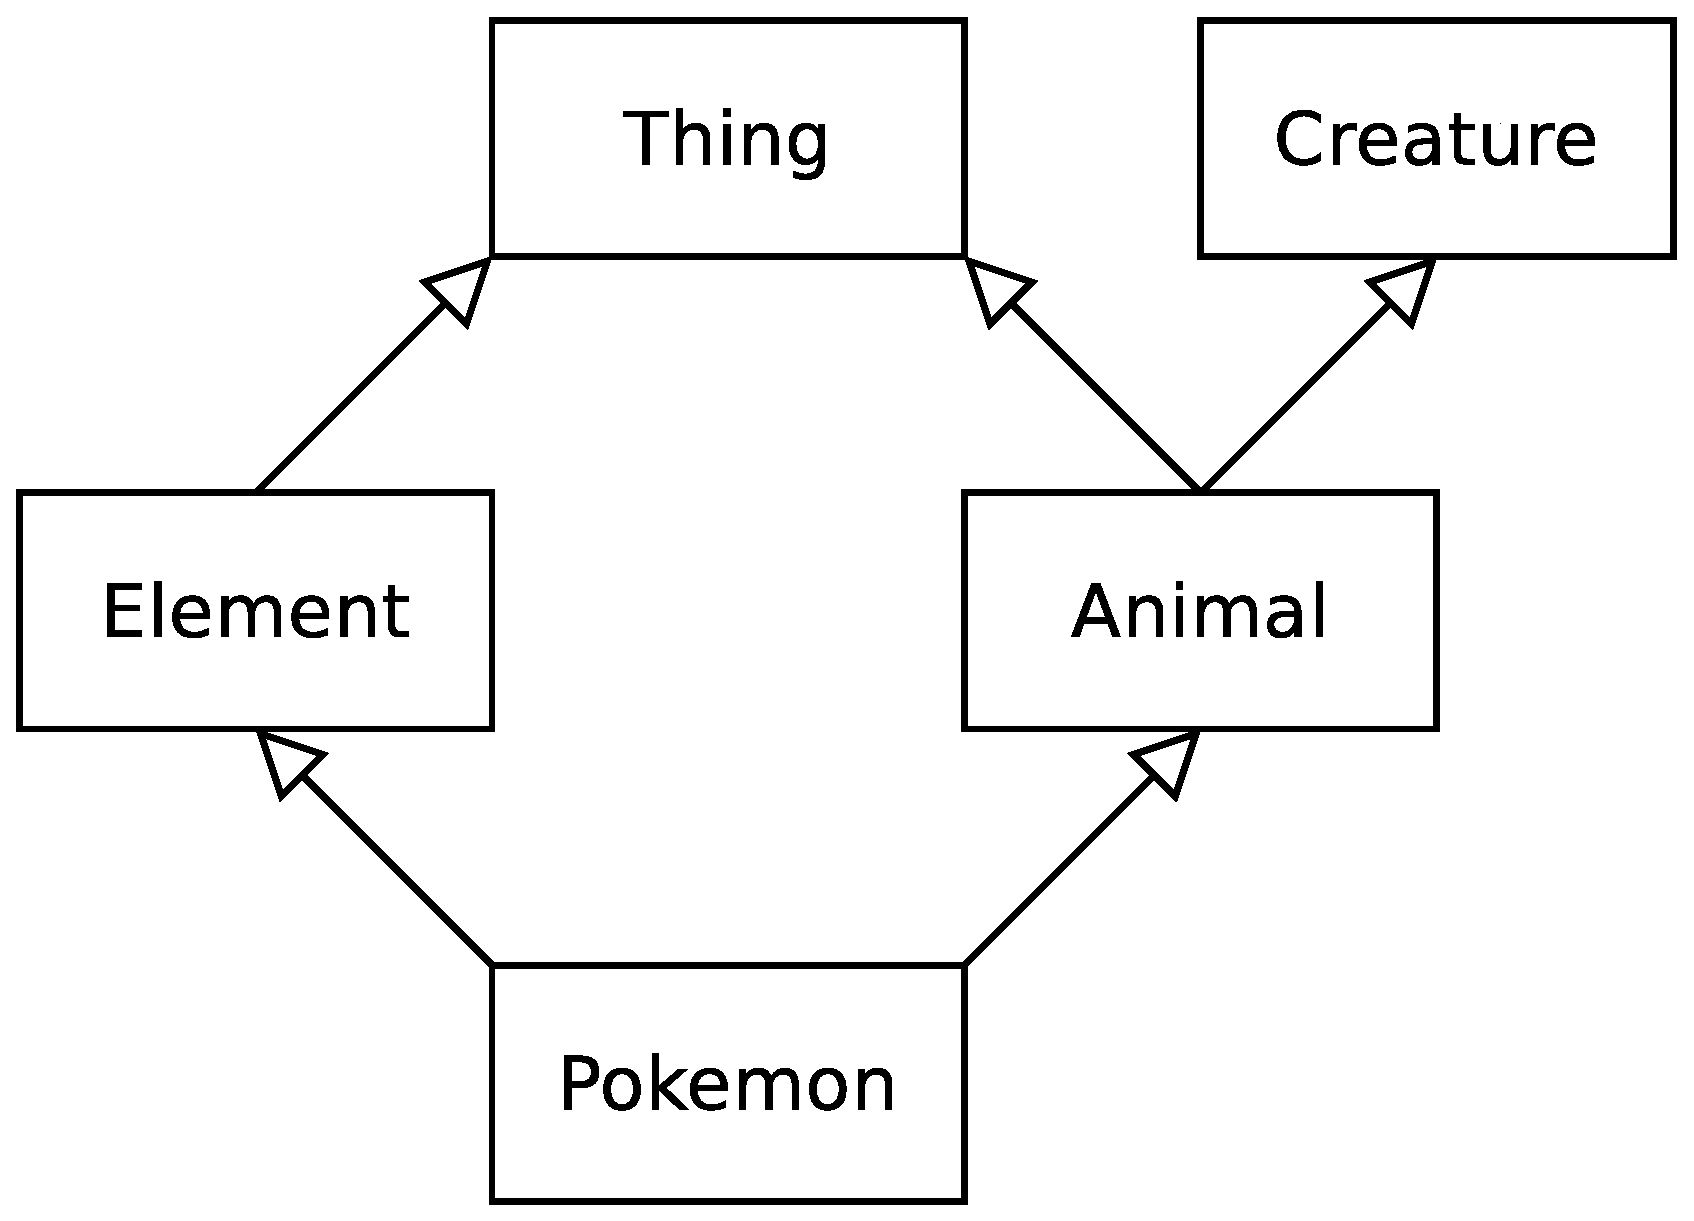
\includegraphics[scale=0.3]{pictures/creature}
 \caption{Vererbungshierarchie mit uneindeutiger Klassenpräzedenz.}
 \label{creature}
\end{figure}

Für Element und Creature sowie Thing und Creature gibt es dann nach den bisher bekannten Regeln kein Constraint, das eine Reihenfolge festlegt. Es ergeben sich drei mögliche Klassenpräzedenzlisten:

(\texttt{Pokemon Element Animal Creature Thing standard-object t})\\
(\texttt{Pokemon Element Animal Thing Creature standard-object t})\\ 
(\texttt{Pokemon Element Thing Animal Creature standard-object t})

CLOS entscheidet sich in dem Fall deterministisch für eine der möglichen Reihenfolgen: diejenige, in der Klassen aus einem Teilbaum möglichst nah beieinander sind. Wenn wir die Klassenhierarchie betrachten, so bilden Element und Thing einen Teilbaum, Animal und Creature einen anderen. CLOS würde demnach die dritte Möglichkeit bevorzugen, in der die Klassen direkt aufeinander folgen.

Falls die Reihenfolge der indirekten Superklassen für das Programm relevant ist, so ist es auch möglich, dies als zusätzliches Constraint anzugeben. Nehmen wir beispielweise an, wir wollen, dass Creature in der Klassenpräzedenzliste vor Thing kommt. Wir können dieses Verhalten erzielen, indem wir die Klassen per Hand zu den ``direkten'' Superklassen in der Klassendefinition von Pokemon hinzufügen:

\begin{lstlisting}
(defclass Pokemon (Element Animal Creature Thing)
  ... )
\end{lstlisting}

Es werden dadurch zwei neue Constraints zur Liste hinzugefügt:

\begin{tabular}{l|c}
 \textbf{Constraint} & \textbf{Regel}\\
 \hline
 \texttt{Animal {\guillemotright} Creature} & 2\\
 \texttt{Creature {\guillemotright} Thing}  & 2\\
\end{tabular}

Diese zusätzlichen Regeln bewirken, dass es nun nur noch eine mögliche Klassenpräzedenzliste gibt:

(\texttt{Pokemon Element Animal Creature Thing standard-object t})\\

Der Fall, dass keine Reihenfolge alle Constraints erfüllt, tritt auf, wenn zwei Oberklassen gegensätzliche Vererbungsreihenfolgen haben. Das ist zum Beispiel gegeben, wenn wir per Hand eine der Klassen Creature oder Thing vor den Klassen Element und Animal in der Klassendefinition anführen:

\begin{lstlisting}
(defclass Pokemon (Element Creature Animal)
  ... )
\end{lstlisting}

Es ergeben sich dann zwei widersprüchliche Constraints:

\begin{tabular}{l|c}
 \textbf{Constraint} & \textbf{Regel}\\
 \hline
 \texttt{Animal {\guillemotright} Creature} & 1\\
 \texttt{Creature {\guillemotright} Animal}  & 2\\
\end{tabular}

In dem Fall signalisiert CLOS einen Fehler, da es keine Klassenpräzedenzliste erstellen kann, die konsistent mit allen Constraints ist.

Eine Beispielimplementierung des Algorithmus für die Berechnung der Klassenpräzedenzliste kann in \cite[S.24f,291f]{amop} nachgelesen werden. Eine der Anforderungen an die Implementierung von Mehrfachbererbung in Racket war, dass sie möglichst ähnlich zu der von CLOS funktionieren soll. Es wird daher die gleiche topologische Sortierung verwendet werden.

CLOS nutzt dann die Klassenpräzedenzliste, um die effektiven Slots zu berechnen:

\begin{lstlisting}
(defun compute-slots (class)
  ... ; conversion to slot object here
  (remove-duplicates
    (apply #'append 
           (mapcar #'class-direct-slots
                   (class-precedence-list class)))
    :key #'slot-definition-name
    :from-end t))
\end{lstlisting}

Es werden die direkten Slots aller Klassen in der Reihenfolge der Präzedenzliste gesammelt und anschließend gleichbenannte Slots entfernt. Dadurch verbleibt nur der Slot der Klasse mit der höchsten Präzedenz in der Liste. Das lässt sich auch leicht auf Definitionen von Racket-Feldern abbilden.

CLOS wandelt die Slot-Definition anschließend noch in Slot-Objekte um. %Diese Umwandlung wird Racket für uns übernehmen.

Mit den CLOS-Konzepten, die wir bisher kennengelernt haben, lässt sich  unser Makro erweitern um Funktionen, die Informationen über die Klasse in Form eines Metaobjektes speichern, die Klassenpräzedenzliste bestimmen und  die effektiven Felder ermitteln. Die Vererbung von Feldern ist damit bereits abgedeckt. Was noch fehlt, ist die Vererbung von Methoden.

\section{Mehrfachvererbung und Methodenkombination}
Analog zu Klassen gibt es auch für Methoden und generische Funktionen Metaobjekte, um eine Übersicht über die relevanten Informationen zu behalten. Eine generische Funktion fasst eine Menge von Methoden mit der gleichen Signatur zusammen und das zugehörige Metaobjekt merkt sich genau diese Dinge: den Namen, die Parameterliste sowie die Methoden, die die generische Funktion implementieren.

\begin{lstlisting}
(defclass standard-generic-function ()
  ((name :initarg :name
         :accessor generic-function-name)
   (lambda-list :initarg :lambda-list
                :accessor generic-function-lambda-list)
   (methods :initform ()
            :accessor generic-function-methods)))
\end{lstlisting}

Die Makros \texttt{defgeneric} und \texttt{defmethod} expandieren dann, analog zu \texttt{defclass}, zu einem Aufruf von \texttt{ensure-generic-function} beziehungsweise \texttt{ensure-method}. \texttt{ensure-generic-function} fügte eine neue generische Funktion zur Liste hinzu während \texttt{ensure-method} die Methode zu einer bestehenden generischen Funktion hinzufügt. Falls es noch keine generische Funktion für die Methode gibt, wird sie erzeugt. In CLOS gibt es zu jeder Methode eine generische Funktion, unabhängig davon, ob der Benutzer sie explizit angibt oder nicht.

Welche Methode bei dem Aufruf einer generischen Funktion ausgeführt wird, hängt von den Argumenten und der Kombinationsart ab. In CLOS ist die Klasse (oder die Klassen), auf die eine Methode spezialisiert ist, Teil der Methodenparameter. 

Falls der Benutzer nichts anderes angibt, geschieht die \emph{standard method combination}, also die Ausführung der spezifischsten Primärmethode und ihrer Ergänzungsmethoden. Sie erfolgt in drei Schritten:
\begin{enumerate}
 \item Bestimmen, welche Methoden anwendbar sind. Methoden sind anwendbar, wenn sie auf die gleiche Klasse wie die auszuführende Methode oder eine ihrer Oberklassen spezialisiert sind.
 \item Sortieren der anwendbaren Methoden nach Präzedenz.
 \item Ausführen der Liste anwendbarer Methoden.
\end{enumerate}

Andere Kombinationsarten werden in AMOP nicht behandelt, aber das gleiche Schema lässt sich sowohl an Ergänzungsmethoden als auch an Methodenkombination anpassen. Sie unterscheiden sich nur darin, welche Methoden anwendbar send, welche Art der Präzedenz für die Sortierung gewählt wird und wie die Methoden anschließend ausgeführt werden (Tabelle \ref{combination}). Falls keine anwendbare Primärmethode gefunden wurde, so wird ein Fehler signalisiert.

\begin{table}[h]
\begin{tabular}{|p{4.7cm}|p{4.5cm}|p{4.5cm}|}
 \hline
 \textbf{Schritt} & \textbf{Ergänzungsmethoden} & \textbf{Methodenkombination}\\\hline
 Bestimmen, welche Methoden anwendbar sind. & Primärmethoden und Ergänzungsmethoden & Primärmethoden \\\hline
 Sortieren der anwendbaren Methoden nach Präzedenz. & Sortieren der Methoden in der Reihenfolge Around, Before, spezifischste Primärmethode, After und innerhalb einer Kategorie nach Klassenpräzedenz & Sortieren der Methoden nach Klassenpräzedenz\\\hline
 Ausführen der Liste anwendbarer Methoden. & Sequentiell & Kombination\\\hline
\end{tabular}
 \caption{Vorgehensweise bei der Methodenkombination.}
 \label{combination}
\end{table}

Auf analoge Weise lässt sich Methodenkombination auch für Racket umsetzen: 
Wir erlauben die Optionen \texttt{define/generic}, \texttt{define/before}, \texttt{define/around} und \texttt{define/after} im \texttt{class}-Makro. Wann immer eine generische Funktion oder Methode angegeben wird, merken wir uns die relevanten Informationen in Form eines Metaobjekts. Und wir sorgen dafür, dass die Methodendefinitionen, für die eine Kombination existiert, durch eine entsprechende Kombinationsmethode ersetzt werden, bevor Racket die Klassendefinition auswertet.

Damit bietet CLOS uns bereits alle Konzepte, die für eine Umsetzung des Entwurfs benötigt werden. Insbesondere die dritte Anforderung lässt sich auf diese Weise sehr elegant umsetzen: da die Funktionalität, die von CLOS übertragen wird, auf analoge Weise implementiert wird, wird sie auch das gleiche Verhalten zeigen.